\documentclass[border=6pt]{standalone}
\usepackage[utf8]{inputenc}\usepackage[T1]{fontenc}\usepackage{amsmath,amsfonts,xcolor,tikz}
\usetikzlibrary{positioning,arrows.meta,calc,fit,backgrounds}
\begin{document}
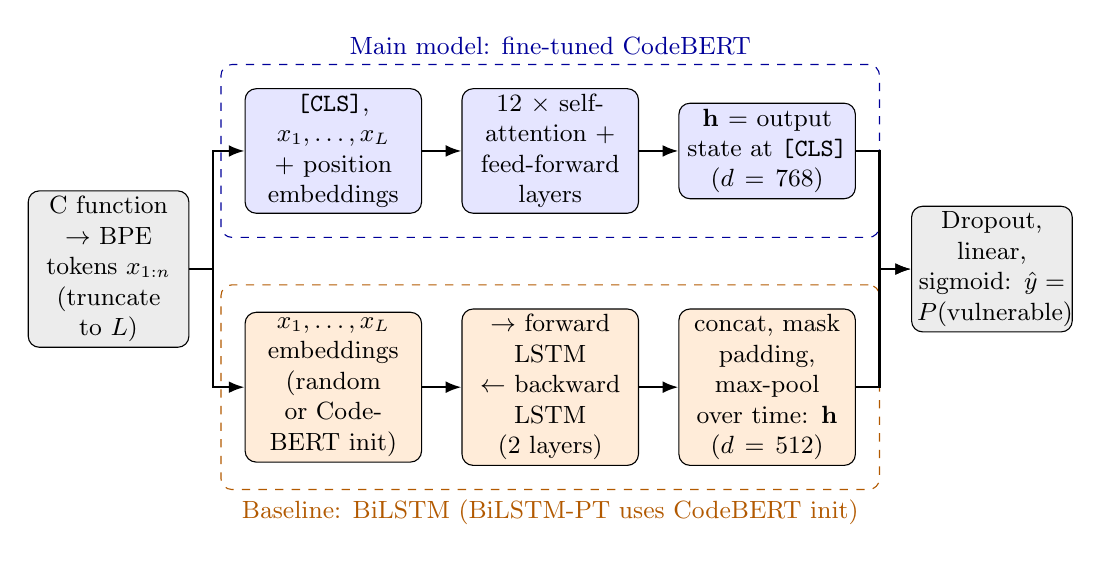
\begin{tikzpicture}[
      node distance=5mm,
      box/.style={draw, rounded corners, align=center, minimum height=11mm, text width=2.1cm, font=\small, inner sep=2pt},
      main/.style={box, fill=blue!10},
      base/.style={box, fill=orange!15},
      io/.style={box, fill=gray!15, text width=1.9cm},
      arr/.style={-{Latex[length=2mm]}, thick},
      grp/.style={draw, rounded corners, dashed, inner sep=3mm}
    ]
    % shared input
    \node[io] (tok) {C function $\to$ BPE tokens $x_{1:n}$ (truncate to $L$)};

    % CodeBERT branch
    \node[main, right=7mm of tok, yshift=15mm] (m1) {\texttt{[CLS]}, $x_1,\dots,x_L$ + position embeddings};
    \node[main, right=of m1] (m2) {12 $\times$ self-attention + feed-forward layers};
    \node[main, right=of m2] (m3) {$\mathbf{h}=$ output state at \texttt{[CLS]} ($d=768$)};

    % BiLSTM branch
    \node[base, right=7mm of tok, yshift=-15mm] (b1) {$x_1,\dots,x_L$ embeddings (random or CodeBERT init)};
    \node[base, right=of b1] (b2) {$\rightarrow$ forward LSTM\\$\leftarrow$ backward LSTM\\(2 layers)};
    \node[base, right=of b2] (b3) {concat, mask padding, max-pool over time: $\mathbf{h}$ ($d=512$)};

    % shared output
    \node[io, anchor=west] (out) at ($(m3.east)!0.5!(b3.east)+(7mm,0)$) {Dropout, linear, sigmoid: $\hat{y}=P(\text{vulnerable})$};

    % arrows
    \draw[arr] (tok.east) -- ++(3mm,0) |- (m1.west);
    \draw[arr] (tok.east) -- ++(3mm,0) |- (b1.west);
    \draw[arr] (m1) -- (m2);
    \draw[arr] (m2) -- (m3);
    \draw[arr] (b1) -- (b2);
    \draw[arr] (b2) -- (b3);
    \draw[arr] (m3.east) -- ++(3mm,0) |- (out.west);
    \draw[arr] (b3.east) -- ++(3mm,0) |- (out.west);

    \begin{scope}[on background layer]
      \node[grp, draw=blue!60!black, fit=(m1)(m2)(m3),
            label={[font=\small, text=blue!60!black]above:Main model: fine-tuned CodeBERT}] {};
      \node[grp, draw=orange!70!black, fit=(b1)(b2)(b3),
            label={[font=\small, text=orange!70!black]below:Baseline: BiLSTM (BiLSTM-PT uses CodeBERT init)}] {};
    \end{scope}
  \end{tikzpicture}
\end{document}
